\subsection{More about Refraction}

Refraction occurs because the \textbf{speed of light waves} is different in each substance. The amount of refraction \underline{depends on the speed of the waves} in each substance.

\begin{enumerate}
    \item Consider a wavefront of light wave when it \textbf{passes across a straight boundary} into a transparent substance.
        \begin{center}
            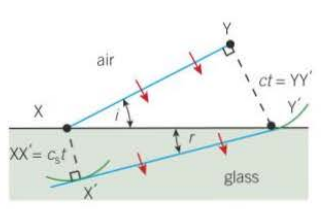
\includegraphics[width=5cm]{img/refraction}
        \end{center}
    \item The \textbf{wavefront} moves from $XY$ to $X'Y'$ in time $t$. The wavefront moves
        \begin{itemize}
            \item A distance $ct$ from $Y$ to $Y'$
            \item A distance $c_st$ from $X$ to $X'$
        \end{itemize}
\end{enumerate}
This gives up equations
\begin{align*}
    \begin{cases}
        ct&=XY'\sin i\\
        c_st&=XY'\sin r
    \end{cases}
\end{align*}

Rearranging gives \textbf{Snell's law} - the smaller the speed of light is in a substance, the greater the refractive index of the substance.
$$n_s=\frac{\sin i}{\sin r}=\frac{c}{c_s}$$

For refraction at a boundary between two transparent substances:
$$n_1\sin\theta_1=n_2\sin\theta_2$$

\subsubsection*{Refraction of White Light}
We can use a \textbf{prism} to split a beam of white light into colours of the spectrum
\begin{itemize}
    \item Light is composed of light with a \textbf{continuous range of wavelengths}.
    \item The shorter the wavelength, the greater the amount of refraction.
    \item So each colour of light is refracted by a different amounts.
\end{itemize}
